\documentclass[journal,12pt,twocolumn]{IEEEtran}
%
\makeatletter
\makeatother
\usepackage{setspace}
\usepackage{gensymb}
\usepackage{xcolor}
\usepackage{caption}
%\usepackage{stackengine}
%\usepackage{subcaption}
%\doublespacing
\singlespacing



\usepackage{graphicx}
\graphicspath{ {./images}  }
%\usepackage{amssymb}
%\usepackage{relsize}
\usepackage[cmex10]{amsmath}
\usepackage{mathtools}
%\usepackage{amsthm}
%\interdisplaylinepenalty=2500
%\savesymbol{iint}
%\usepackage{txfonts}
%\restoresymbol{TXF}{iint}
\usepackage{wasysym}
\usepackage{amsthm}
\usepackage{mathrsfs}
\usepackage{txfonts}
\usepackage{stfloats}
\usepackage{cite}
\usepackage{cases}
\usepackage{mathtools}
\usepackage{subfig}
\usepackage{enumerate}	
\usepackage{enumitem}
\usepackage{amsmath}
%\usepackage{xtab}
\usepackage{longtable}
\usepackage{multirow}
%\usepackage{algorithm}
%\usepackage{algpseudocode}
\usepackage{enumitem}
\usepackage{mathtools}
%\usepackage{iithtlc}
%\usepackage[framemethod=tikz]{mdframed}
\usepackage{listings}
\usepackage{listings}
    \usepackage[latin1]{inputenc}                                 %%
    \usepackage{color}                                            %%
    \usepackage{array}                                            %%
    \usepackage{longtable}                                        %%
    \usepackage{calc}                                             %%
    \usepackage{multirow}                                         %%
    \usepackage{hhline}                                           %%
    \usepackage{ifthen}                                           %%
  %optionally (for landscape tables embedded in another document): %%
    \usepackage{lscape}     



%\usepackage{stmaryrd}


%\usepackage{wasysym}
%\newcounter{MYtempeqncnt}
\DeclareMathOperator*{\Res}{Res}
%\renewcommand{\baselinestretch}{4}
%\setcounter{secnumdepth}{4}
\renewcommand\thesection{\arabic{section}}
\renewcommand\thesubsection{\thesection.\arabic{subsection}}
\renewcommand\thesubsubsection{\thesubsection.\arabic{subsubsection}}
%\renewcommand\thesubsubsubsection{\thesubsubsection.\arabic{subsubsubsection}}

%\renewcommand\thesectiondis{\arabic{section}}
%\renewcommand\thesubsectiondis{\thesectiondis.\arabic{subsection}}
%\renewcommand\thesubsubsectiondis{\thesubsectiondis.\arabic{subsubsection}}
%\renewcommand\thesubsubsubsectiondis{\thesubsubsectiondis.\arabic{subsubsubsection}}
% correct bad hyphenation here
\hyphenation{op-tical net-works semi-conduc-tor}

%\lstset{
%language=C,
%frame=single, 
%breaklines=true
%}

%\lstset{
	%%basicstyle=\small\ttfamily\bfseries,
	%%numberstyle=\small\ttfamily,
	%language=Octave,
	%backgroundcolor=\color{white},
	%%frame=single,
	%%keywordstyle=\bfseries,
	%%breaklines=true,
	%%showstringspaces=false,
	%%xleftmargin=-10mm,
	%%aboveskip=-1mm,
	%%belowskip=0mm
%}

%\surroundwithmdframed[width=\columnwidth]{lstlisting}
\def\inputGnumericTable{}                                 %%

\lstset{
%language=python,
frame=single, 
breaklines=true,
columns=fullflexible
}

 

\begin{document}
%

\theoremstyle{definition}
\newtheorem{theorem}{Theorem}[section]
\newtheorem{problem}{Problem}
\newtheorem{proposition}{Proposition}[section]
\newtheorem{lemma}{Lemma}[section]
\newtheorem{corollary}[theorem]{Corollary}
\newtheorem{example}{Example}[section]
\newtheorem{definition}{Definition}[section]
%\newtheorem{algorithm}{Algorithm}[section]
%\newtheorem{cor}{Corollary}
\newcommand{\BEQA}{\begin{eqnarray}}
\newcommand{\EEQA}{\end{eqnarray}}
\newcommand{\define}{\stackrel{\triangle}{=}}

\bibliographystyle{IEEEtran}
%\bibliographystyle{ieeetr}

\providecommand{\nCr}[2]{\,^{#1}C_{#2}} % nCr
\providecommand{\nPr}[2]{\,^{#1}P_{#2}} % nPr
\providecommand{\mbf}{\mathbf}
\providecommand{\pr}[1]{\ensuremath{\Pr\left(#1\right)}}
\providecommand{\qfunc}[1]{\ensuremath{Q\left(#1\right)}}
\providecommand{\sbrak}[1]{\ensuremath{{}\left[#1\right]}}
\providecommand{\lsbrak}[1]{\ensuremath{{}\left[#1\right.}}
\providecommand{\rsbrak}[1]{\ensuremath{{}\left.#1\right]}}
\providecommand{\brak}[1]{\ensuremath{\left(#1\right)}}
\providecommand{\lbrak}[1]{\ensuremath{\left(#1\right.}}
\providecommand{\rbrak}[1]{\ensuremath{\left.#1\right)}}
\providecommand{\cbrak}[1]{\ensuremath{\left\{#1\right\}}}
\providecommand{\lcbrak}[1]{\ensuremath{\left\{#1\right.}}
\providecommand{\rcbrak}[1]{\ensuremath{\left.#1\right\}}}
\theoremstyle{remark}
\newtheorem{rem}{Remark}
\newcommand{\sgn}{\mathop{\mathrm{sgn}}}
\providecommand{\abs}[1]{\left\vert#1\right\vert}
\providecommand{\res}[1]{\Res\displaylimits_{#1}} 
\providecommand{\norm}[1]{\lVert#1\rVert}
\providecommand{\mtx}[1]{\mathbf{#1}}
\providecommand{\mean}[1]{E\left[ #1 \right]}
\providecommand{\fourier}{\overset{\mathcal{F}}{ \rightleftharpoons}}
%\providecommand{\hilbert}{\overset{\mathcal{H}}{ \rightleftharpoons}}
\providecommand{\system}{\overset{\mathcal{H}}{ \longleftrightarrow}}
	%\newcommand{\solution}[2]{\textbf{Solution:}{#1}}
\newcommand{\solution}{\noindent \textbf{Solution: }}
\providecommand{\dec}[2]{\ensuremath{\overset{#1}{\underset{#2}{\gtrless}}}}
\DeclarePairedDelimiter{\ceil}{\lceil}{\rceil}
%\numberwithin{equation}{subsection}
\numberwithin{equation}{section}
%\numberwithin{problem}{subsection}
%\numberwithin{definition}{subsection}
%\makeatletter
%\@addtoreset{figure}{section}
%\makeatother

\let\StandardTheFigure\thefigure
%\renewcommand{\thefigure}{\theproblem.\arabic{figure}}
%\renewcommand{\thefigure}{\thesection}


%\numberwithin{figure}{subsection}

%\numberwithin{equation}{subsection}
%\numberwithin{equation}{section}
%\numberwithin{equation}{problem}
%\numberwithin{problem}{subsection}
%\numberwithin{problem}{section}
%%\numberwithin{definition}{subsection}
%\makeatletter
%\@addtoreset{figure}{problem}
%\makeatother
%\makeatletter
%\@addtoreset{table}{problem}
%\makeatother

\let\StandardTheFigure\thefigure
\let\StandardTheTable\thetable
%%\renewcommand{\thefigure}{\theproblem.\arabic{figure}}
%\renewcommand{\thefigure}{\theproblem}

%%\numberwithin{figure}{section}

%%\numberwithin{figure}{subsection}



\def\putbox#1#2#3{\makebox[0in][l]{\makebox[#1][l]{}\raisebox{\baselineskip}[0in][0in]{\raisebox{#2}[0in][0in]{#3}}}}
     \def\rightbox#1{\makebox[0in][r]{#1}}
     \def\centbox#1{\makebox[0in]{#1}}
     \def\topbox#1{\raisebox{-\baselineskip}[0in][0in]{#1}}
     \def\midbox#1{\raisebox{-0.5\baselineskip}[0in][0in]{#1}}



\title{ 
%	\logo{
Digit Recognition using CNN
%	}
}



\author{Ashish, G V V 
Sharma$^{*}$% <-this % stops a space
\thanks{*The authors are with the Department
of Electrical Engineering, Indian Institute of Technology, Hyderabad
502285 India e-mail:  gadepall@iith.ac.in.}
}


% make the title area
\maketitle

\tableofcontents

\bigskip
%
\begin{abstract}
%\boldmath
This manual provides a brief description on how to implement a Convolutional Neural Network from scratch and use it to recognise a hand written digit.
\end{abstract}

%\IEEEpeerreviewmaketitle
%
\section{Objective}
%\subsection{Transmitter}
%\begin{equation}
%m \rightarrow\boxed	{BPSK}\rightarrow\boxed	{\uparrow T_{sym}}\rightarrow C	
%\end{equation}
%
%  Let bit stream was $m$, $xc$ will be mapped sequence and $C$ will be upsampled by $T_{sym}$
% Where $T_{sym}$ is the samples per symbol. 
%\begin{equation}
%X=P \circledast C
%\end{equation} where $P$ is the shape of the pulse. And defined as,
%\begin{equation}
%    P =
%    \begin{cases}
%      1 & 0\leq t\leq 99 \\
%      0        & otherwise
%    \end{cases}
%  \end{equation}
%\subsection{Receiver}
Our objective is to implement and train a CNN on the standard MNIST database and use those trained parameters to recognise our own hand written digits.
%\begin{equation}
%Y_k(m)= X_k + V_k(m), \quad k = 1,\dots,N, m = 1 ,\dots,M.
%\end{equation} 
%where $X_k$ is the transmitted symbol in the $k$th time slot and $V_k(m) \sim \mathcal{N}\brak{0,\sigma^2} $. 
%The decision variable for the $k$th symbol 
%is 
%\cite{time_offset}
%\begin{align}
%U_k&=Y_{k-1}\brak{\frac{M}{2}}\sbrak{Y_{k}\brak{M}-Y_{k-1}\brak{M}}
%\begin{align}
%U_k=\frac{1}{N}\sum^{N}_{i=1}Y_{k-i}\brak{\frac{M}{2}}\sbrak{Y_{k-i+1}\brak{M}-Y_{k-i}%\brak{M}}
%\end{align}
%\end{align}
%
\section{Training Dataset}
The MNIST database used for training this CNN is available at the following link. Download all the four files in the folder where you want to train the CNN
\begin{lstlisting}
http://yann.lecun.com/exdb/mnist/
\end{lstlisting}
\section{About CNN}
A CNN is a combination of convolutional filters and fully connected Multi Layer Perceptron (MLP) with backpropagation implemented to update the parameters during the  training phase.
\linebreak
\linebreak
There are four main operations in the ConvNet:\linebreak
1)Convolution
2)Non Linearity (ReLU)
3)Pooling or Sub Sampling
4)Fully connected MLP for Classification

\subsection{Architecture Used}
The detailed CNN architecture is used classification of handwritten digits is presented in Fig.1. The first block Image represents training image from MNIST database. All the images in the MNIST database are of the dimension 28*28 pixels.\linebreak
\linebreak
In brief, the architecture is:

INPUT - CONV1 - RELU - CONV2 - RELU- MAXPOOL - FC1 - OUT
%\begin{figure}
%\begin{center}
%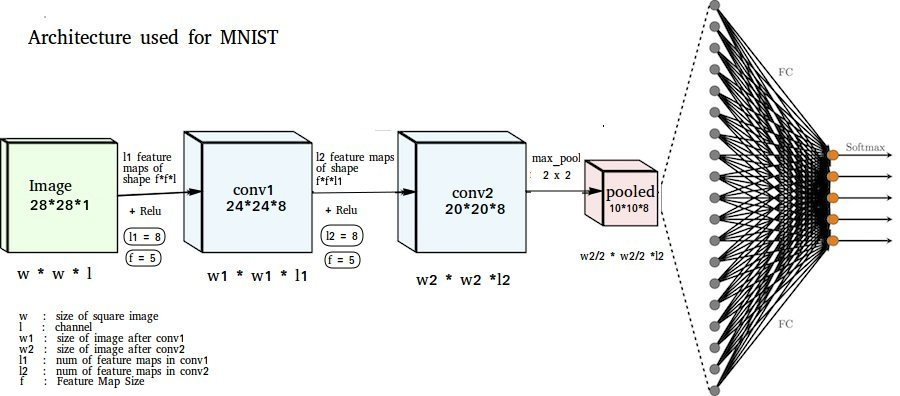
\includegraphics[width=\columnwidth]{./figs/archi_mnist.jpg}
%\end{center}
%\caption{CNN Architecture  }
%\label{fig:arch}
%\end{figure}
\subsection{Hyperparameters Initialisation}
CNN is initialised with the following hyperparameters:

NumOutput=10,
LearningRate=0.01,	
ImgWidth=28,
ImgDepth=1,
FilterSize=5,
NumFilt1=8,
NumFilt2=8,
BatchSize=20,
NumEpochs=2, 
MU=0.95 

Filter size represents the dimension of convolutional filters. Here, the dimension of convolutional filters in both the layers is 5*5. The number of filters in each layer is 8. Epochs represent the number of times the network is allowed to see an image in the training set. The hyperparameter Mu represents momentum in the momentum gradient descent algorithm implemented to update the parameters.

\subsection{Parameters Initialisation}
The parameters of the CNN are: Filter weights of Convolutional Layer 1, Layer 2 and their corrosponding biases, Weights of edges in fully connected layer and the biases of each node in output layer. All the biases are initialised to zero (for both convolutional filters and fully connected layer). The filter weights are initialised using lecun normal distribution. The weights of edges in fully connected layer are initialised using uniform distribution.
\linebreak
\subsubsection{Lecun Normal Distribution}
It draws samples from a truncated normal distribution centered on 0 with stddev=sqrt(1 /fanIn) where fanIn is the number of input units in the weight tensor.

\subsection{Back Propagation}
Back Propagation algorithm is implemented to update each of the parameters above during the training phase after passing each batch of images. To know more about Back Propagation Algorithm, refer the following tutorial:
\begin{lstlisting}
https://pdfs.semanticscholar.org/5d79/11c93ddcb34cac088d99bd0cae9124e5dcd1.pdf\end{lstlisting}

\section{Training}
The CNN initialised above is trained on the available MNIST database. This database also has a separate set for testing the trained network. We can use this set to compute the accuracy of the trained network. The code for training the database can be obtained by cloning the all the files in following github link in the folder where MNIST database is stored.
\begin{lstlisting}
https://github.com/EE15BTECH11025/cnn_implementation
\end{lstlisting}

The network can be trained and accuracy can be computed by running the train.py file. The number of images from the database to be used for training (upto 50000) and testing (upto 10000) can be changed by changing the corrosponding variables in the code and accuracy check can be performed. Note that generally the performance of the network increases as we increase the number of training images as the network becomes more 'trained' to take an accurate decision. The parameters of the trained network are stored in pickle file denoted by PickleFile variable in the code.

\section{Testing}
Our task now is to recognise our own hand written digits using the parameters of the trained network. For this, we require the images of our own hand written digits to be given as input. One important note to make here is that the input image given to the network should be of size 28*28 pixels as the parameters trained corrospond to MNIST database in which each image is of size 28*28 pixels.

The pickle file trained.pickle contains the parameters when the network is trained on all the available images in the MNIST Database. We can use this pickle file or the file in which we stored parameters after training the network by changing the variable PickleFile in test.py

The test.py file can be used for testing the network. As an example, I have stored resized (28*28 pixels) images of my handwritten digits in 28pix folder and giving them as input to test the acurracy of network (using trained.pickle as pickle file). The prediction for each image and their corrosponding probabilities are presented in Fig.2. 

%\pagebreak
\section{Figures}
\begin{figure}[!h]
\begin{center}
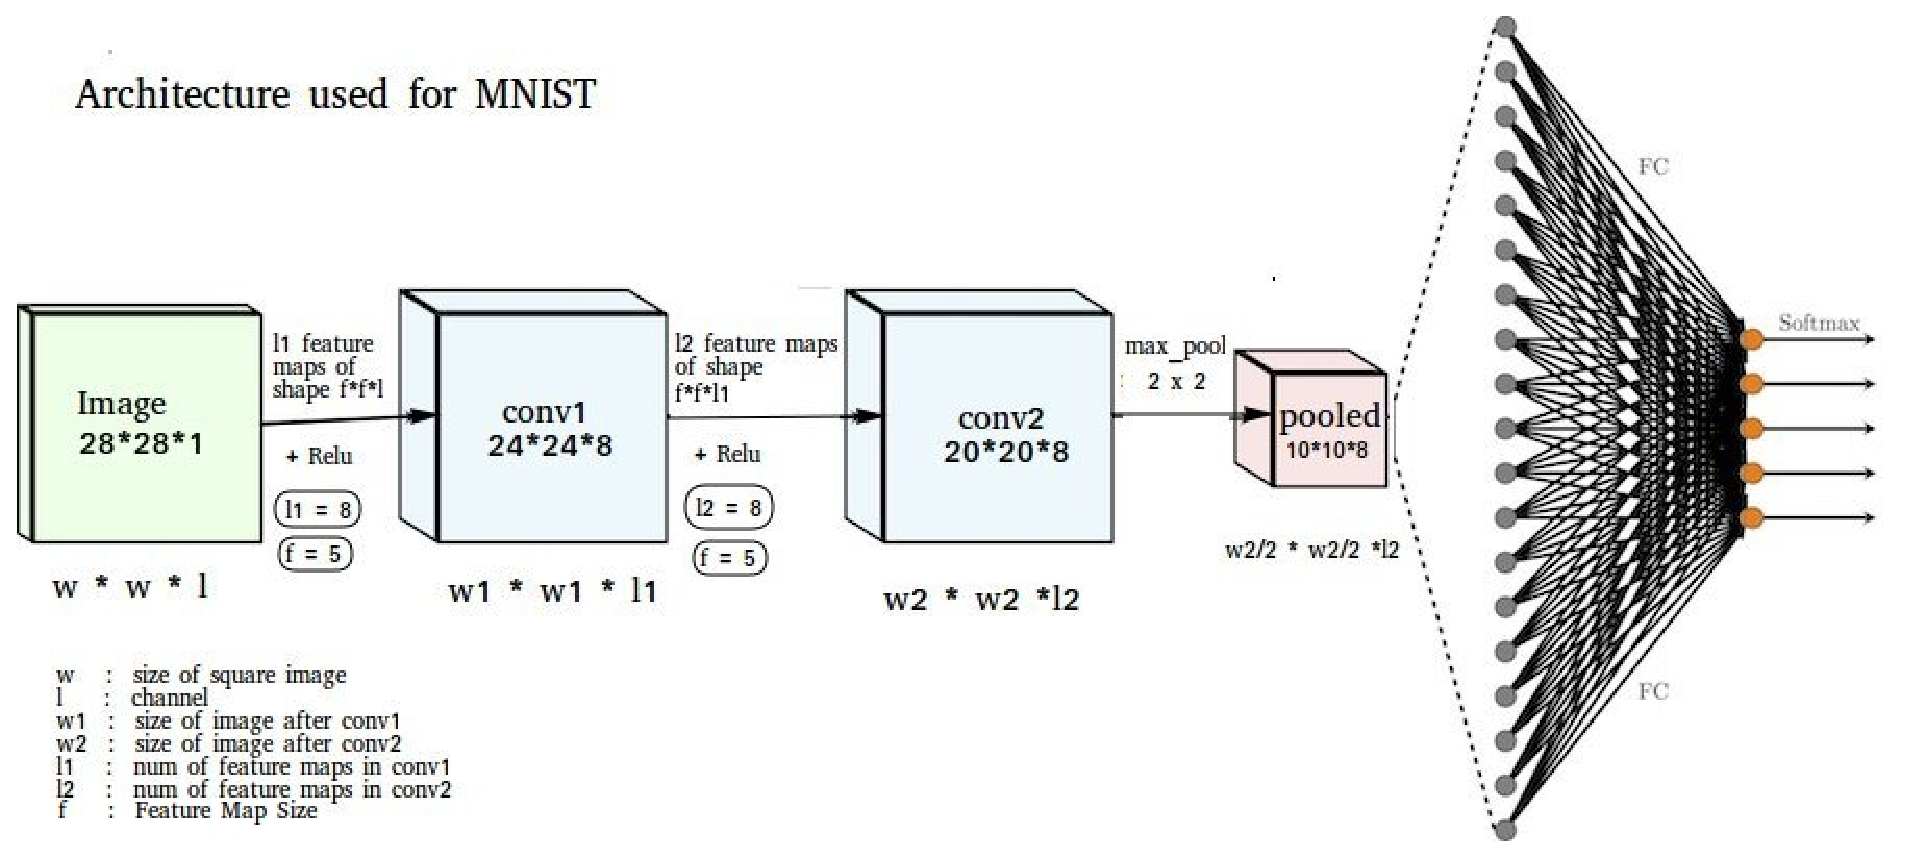
\includegraphics[width=6.0in,angle=90]{./figs/archi_mnist.eps}
%\includegraphics[width = 7cm, height = 10cm]{./figs/app}
\end{center}
\caption{}
\label{fig:cnn_archi}
\end{figure}

\begin{figure}[!h]
\begin{center}
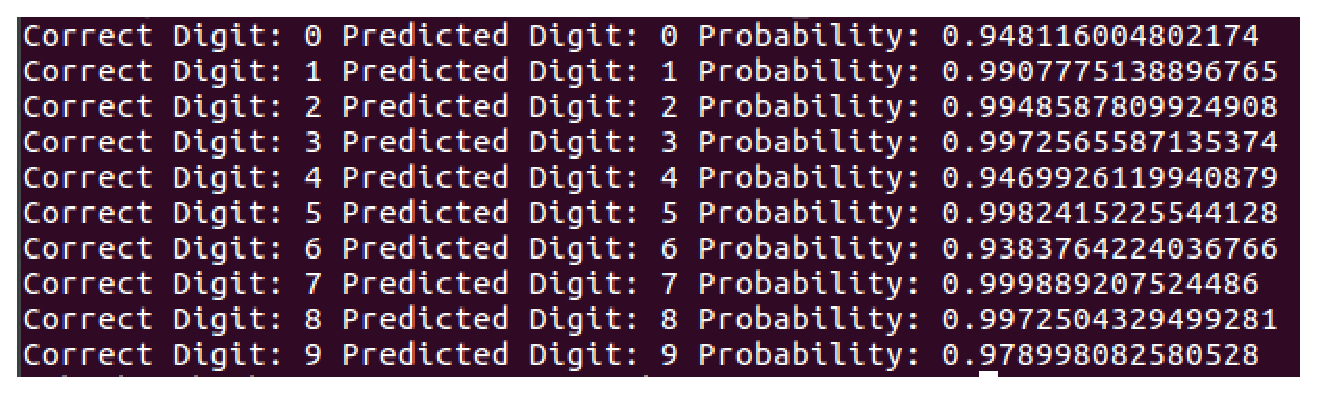
\includegraphics[width=4.0in]{./figs/test_result.eps}
%\includegraphics[width = 7cm, height = 10cm]{./figs/app}
\end{center}
\caption{}
\label{fig:results}
\end{figure}



\end{document}

